\documentclass[11pt]{article}
\usepackage[utf8]{inputenc}
\usepackage[margin=1in]{geometry}
\usepackage{graphicx}
\usepackage{booktabs}
\usepackage{hyperref}
\usepackage{lineno}
\usepackage{amsmath}
\hypersetup{colorlinks=true, linkcolor=blue, urlcolor=blue, citecolor=blue}
\linenumbers

\title{From Reporting Patterns to Extracted Magnitudes: Full-Text LLM Mining
Recovers the Direction but Inflates the Magnitude of Stress-Related Brain Change
Across 384 Studies}

\author{Byeongsoo Kang\thanks{SYSOFT. Corresponding author: shoo99@gmail.com}}
\date{2026}

\begin{document}
\maketitle

\begin{abstract}
\textbf{Background.} Our companion abstract-level scoping review of 9{,}585
studies (Research Square, rs-9884522) reported \emph{literature reporting
patterns}---directional counts of how chronic stress changes the brain---and
explicitly flagged that these are not pooled effect sizes. A recurring question
is whether those count-based patterns survive when the actual numeric effect
sizes are extracted from full text.

\textbf{Methods.} We applied a hybrid pipeline---regex pre-extraction of
numeric candidates from PMC Open Access full texts, followed by LLM mapping
(Qwen3.6-35B-A3B, a 35B Mixture-of-Experts model run under llama.cpp at
temperature 0) of each candidate to a (brain region, metric, direction, value,
measure type) record. After a paper-level stress/disorder context filter and a
sentence-level noise filter (removing laterality comparisons, ratios,
coordinate/cluster statistics, protective-factor and task-performance
correlations), we synthesized direction and magnitude per brain region $\times$
metric class. Because extraction is at the sentence level, the \emph{study}---not
the sentence---was the primary unit: we collapsed entries to one majority-vote
direction per study $\times$ region $\times$ metric before an exact binomial
sign test. A blinded rule-based check on 300 sentences estimated direction
accuracy. This is an effect-size \emph{synthesis}, not an inverse-variance
meta-analysis: per-study sample sizes were recoverable in only $\sim$6\% of
records.

\textbf{Results.} The cleaned set comprised 787 effect-bearing sentences from 384
studies (1{,}490 region-mapped entries); blinded validation gave 94\% direction
accuracy with symmetric errors. At the \emph{study level}, structural decrease
remained significant for the hippocampus (56 vs.\ 12 studies, sign
$p=6\times10^{-8}$) and striatum (6 vs.\ 0, $p=0.03$), but \emph{not} for the
amygdala (24 vs.\ 14, $p=0.14$)---the amygdala's entry-level significance was an
artifact of within-study clustering. Functional measures showed \emph{no} clear
directional signal in any region (amygdala 46 vs.\ 32 studies, $p=0.14$;
hippocampus 18 vs.\ 15, $p=0.73$). r-type correlations with stress/severity
centered near $r\approx-0.30$ for amygdala, hippocampus and ACC. Crucially, these
extracted magnitudes ($r\approx-0.3 \approx$ Cohen's $d\approx-0.65$) are
\textbf{3--6$\times$ larger} than the corresponding individual-patient-data
mega-analyses (ENIGMA-PTSD hippocampus $d=-0.17$, amygdala $d=-0.11$), indicating
that the published, extractable literature systematically overstates true effect
magnitudes. Thus full-text mining \textbf{recovers the direction} of the
canonical structural-decrease pattern but \textbf{reproduces its
publication-bias-inflated magnitude}.

\textbf{Conclusions.} Moving from count-based reporting patterns to extracted
effect-size magnitudes confirms the \emph{direction} of stress-related structural
decrease, but benchmarking against consortium mega-analyses shows the extracted
\emph{magnitudes} are inflated several-fold---demonstrating that large-scale LLM
mining of published text can quantify, rather than escape, the field's
publication bias. We are transparent about the pipeline's validated direction
accuracy (94\%), its mapping yield ($\sim$43\%), and the absence of usable sample
sizes for formal pooling; these define the boundary between this synthesis and a
definitive meta-analysis. The list of all included studies is provided as
Supplementary Table~S1.
\end{abstract}

\medskip
\noindent\textbf{Keywords:} chronic stress; brain structure; effect-size
synthesis; full-text mining; LLM extraction; publication bias; effect-size
inflation; mega-analysis benchmarking; hippocampus; amygdala

\section{Introduction}

The chronic stress literature is dominated by a small number of canonical
statements: stress reduces hippocampal volume, increases amygdala reactivity,
and impairs prefrontal function. Our companion study \cite{kang2026scoping}
tested whether such statements hold \emph{quantitatively at scale} by extracting
structured directional labels from 9{,}585 PubMed abstracts using a
397-billion-parameter LLM on a CPU cluster. That work deliberately reported
\emph{reporting patterns}---how often the literature says ``decrease'' vs.\
``increase''---and stressed that abstract-level counts are not pooled effect
sizes; full-text quantitative synthesis was named as the necessary next step.

This paper takes that step. We extract the actual numeric effect sizes (Cohen's
$d$, Hedges' $g$, correlation $r$, $t$/$F$ statistics) from the Results sections
of the PMC Open Access subset of those studies, map each to the brain region and
metric it describes, and ask a single question: \textbf{when we move from
counting directional claims to extracting effect-size magnitudes, do the
abstract-level patterns survive?} We focus on the two patterns most central to
the field---structural decrease, and the structural-vs-functional dissociation
that our abstract-level review argued resolves the ``amygdala increases''
controversy.

We are explicit that this is an effect-size \emph{synthesis}, not a definitive
meta-analysis. Full-text sentences report effect sizes far more often than they
report the per-cell sample sizes needed for inverse-variance weighting; we
therefore lean on study-level directional sign tests and magnitude
distributions, and we benchmark the extracted magnitudes against the largest
individual-patient-data (IPD) mega-analyses of the field---which are, by design,
free of publication bias---so that readers can see not only whether the
direction is recovered but whether the magnitude is trustworthy.

\section{Methods}

\subsection{Corpus and full-text retrieval}
Starting from the 9{,}585-abstract corpus \cite{kang2026scoping}, we mapped
PMIDs to PMC identifiers and retrieved the PMC Open Access full-text XML where
available (4{,}353 articles). Each article's Results section (falling back to the
full body) was parsed from JATS XML.

\subsection{Regex pre-extraction (CPU, no LLM)}
We split each Results section into sentences and, with curated regular
expressions, flagged numeric effect-size candidates ($d$, $g$, $r$, $\beta$,
$t(\cdot)$, $F(\cdot)$, $\eta^2$), confidence intervals, $p$-values, sample sizes
($n=\cdot$), and brain-region mentions. Sentences containing at least one
effect-size candidate were retained, producing the candidate pool for LLM
mapping. This step is deterministic and reproducible
(\texttt{fulltext\_hybrid\_extract.py}).

\subsection{LLM relationship-aware mapping}
Each candidate sentence was sent to a 35B MoE model (Qwen3.6-35B-A3B, llama.cpp,
\texttt{temperature}=0) on the CPU cluster, prompted to return a JSON array in
which each numeric value is mapped to \{brain\_region, metric, direction, value,
measure\_type\} \emph{only if} it quantifies how a brain region's metric changes
\emph{in relation to stress or a stress-related disorder} (patients vs.\
controls, stressed vs.\ non-stressed, or correlation with a stress/severity
measure). The prompt explicitly instructed the model to reject regression
predictors (age, sex, education, medication), task-performance correlations,
scanner/coordinate numbers, and protective-factor effects, and to emit an empty
array when nothing qualifies. Keeping each output small ($<512$ tokens) avoids
the quantization-related JSON failures we observed with long outputs. We
deliberately used a compact 35B MoE model rather than the 397B model used for
abstract-level extraction in the companion study \cite{kang2026scoping}: the
full-text task operates on single pre-filtered sentences with a tightly
constrained output schema, for which the smaller model was sufficient at
temperature 0 while remaining tractable on a CPU-only cluster. The exact prompt
is reproduced verbatim in Appendix~A.

\subsection{Two-stage noise filtering}
A \emph{paper-level} filter restricted mapping to studies whose corpus context is
stress/disorder-related. A subsequent \emph{sentence-level} filter (applied at
synthesis) removed residual noise classes that the model occasionally mismapped:
left-vs-right laterality comparisons, volume \emph{ratios}, sentences dominated by
MNI coordinates / cluster-size / TFCE statistics, protective-factor sentences,
and cognitive-task-performance correlations. We report results both before and
after this filter for transparency.

\subsection{Synthesis (not meta-analysis)}
For each (region, metric-class) we tabulated decrease/increase/null counts.
Because extraction is at the sentence level and a single study can contribute
several entries, \textbf{the primary unit of analysis is the study, not the
sentence}: within each study $\times$ region $\times$ metric we assigned a single
direction by majority vote (ties excluded) and computed an exact two-sided
binomial sign test ($H_0$: $p=0.5$) over study-level directions. We additionally
report the entry-level test as a sensitivity analysis, noting that entry-level
$p$-values are anti-conservative because sentences within a study are not
independent. For $r$-type entries we summarized the magnitude distribution
(median, IQR). Metric class was structural (volume, GMV, thickness, FA, density)
vs.\ functional (activation, connectivity, BOLD, ALFF). Because usable sample
sizes appeared in only $\sim$6\% of records, no inverse-variance random-effects
pooling was attempted; we frame the output as a directional + magnitude
synthesis and benchmark magnitudes externally (\S3.6).

\subsection{Extraction validation}
To estimate extraction accuracy, we drew a sample of 300 mapped sentences and,
blind to the model's output, derived an independent ``silver'' direction label
from explicit lexical cues in each sentence (e.g.\ \emph{reduced/smaller/lower}
$\to$ decrease; \emph{increased/greater/higher} $\to$ increase; sentences without
an unambiguous cue were excluded). Against this label we computed the model's
direction accuracy and a decrease/increase confusion matrix, the latter because
all downstream sign tests depend on direction being unbiased.

\section{Results}

\subsection{Extraction yield and cleaning}
Of the stress-context candidate sentences, 933 yielded a confident LLM mapping
(\emph{mapping yield} $\approx$ 43\%; the remainder were empty arrays, dominated
by ``no significant'' statements and non-qualifying numbers). We use
\emph{mapping yield} rather than \emph{recall} because the denominator is the
regex candidate pool and the true set of effect-bearing sentences is not
independently known. The sentence-level noise filter removed 146 sentences
($\sim$16\%), leaving a cleaned set of \textbf{787 sentences from 384 studies,
yielding 1{,}490 region-mapped effect-size entries}. The cleaning removed noise
roughly symmetrically and left the headline directions intact.

\begin{figure}[t]
\centering
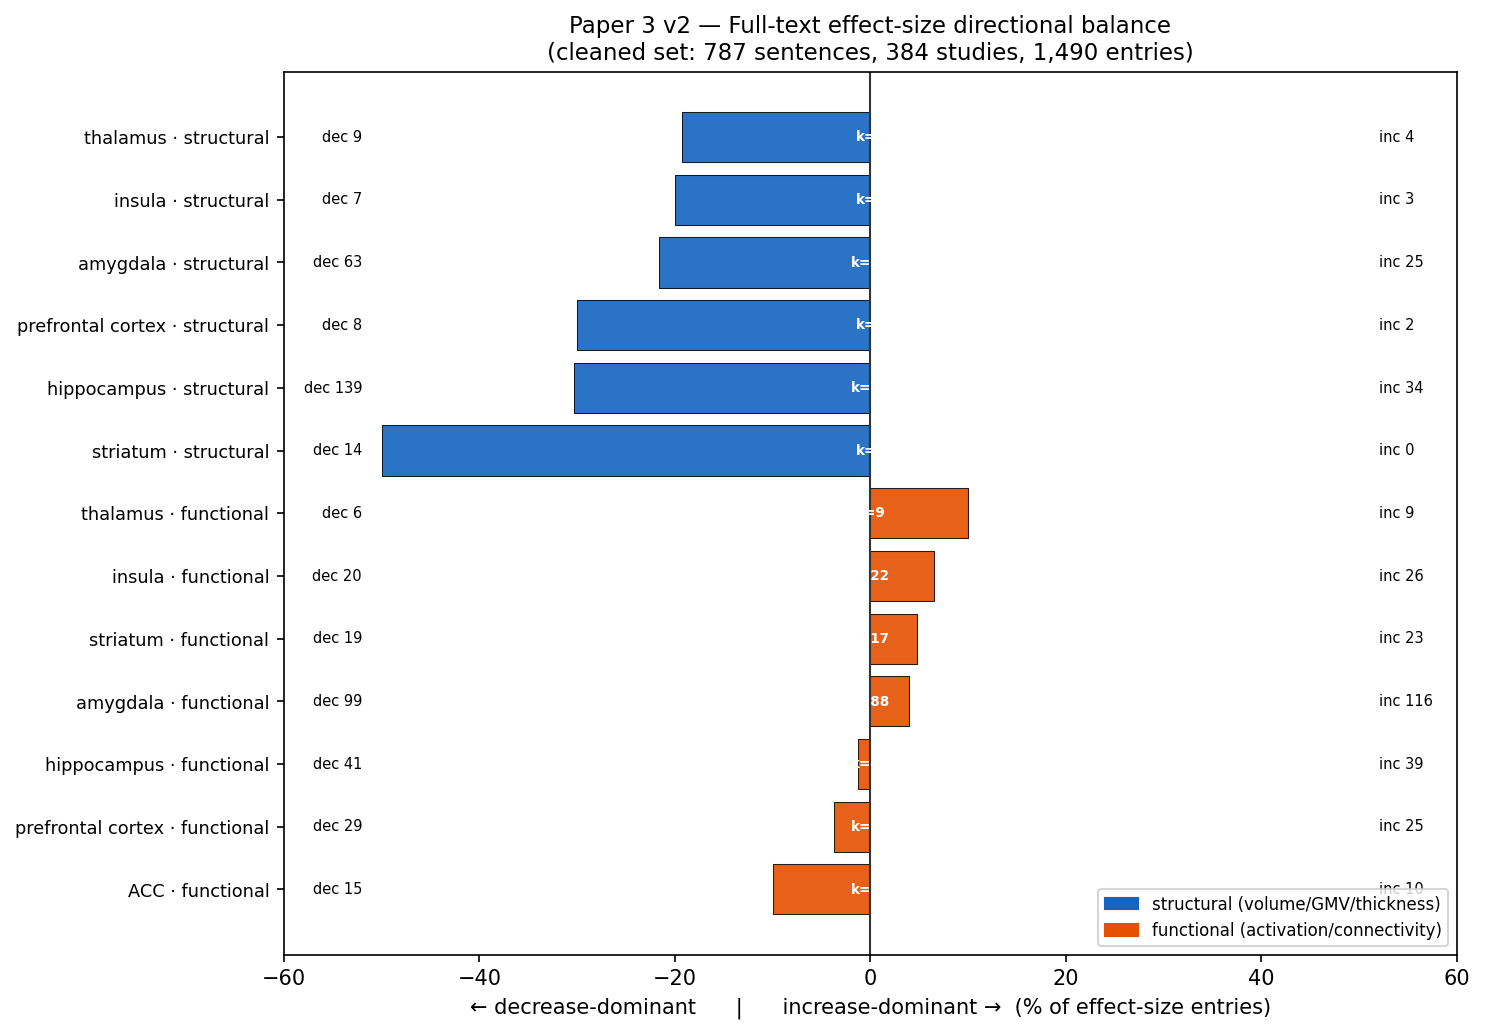
\includegraphics[width=\linewidth]{figures_v2/v2_fig1_directional_balance.png}
\caption{Full-text effect-size directional balance per brain region $\times$
metric class (cleaned set: 787 sentences, 384 studies, 1{,}490 entries). Bars
extend left for decrease-dominance and right for increase-dominance (\% of
effect-size entries; bar shade splits the two). $k$ = number of contributing
studies. Structural metrics (blue) are decrease-dominant in every region (robust
at the study level for hippocampus and striatum); functional metrics (orange)
carry no significant directional signal. Bar lengths are descriptive proportions
of effect-size entries, not pooled effects; significance refers to the
study-level sign tests in Table~\ref{tab:dir}.}
\label{fig:balance}
\end{figure}

\begin{table}[t]
\centering
\caption{Directional synthesis per brain region $\times$ metric class (cleaned
full-text effect sizes). The \textbf{study-level} sign test (majority-vote
direction per study) is the primary statistic; entry-level counts and $p$-values
are shown for completeness but are anti-conservative due to within-study
clustering. Sign test: exact two-sided binomial, ties/nulls excluded.}
\label{tab:dir}
\begin{tabular}{llrrr@{\hskip 12pt}rrr}
\toprule
 & & \multicolumn{3}{c}{Study-level} & \multicolumn{3}{c}{Entry-level} \\
\cmidrule(lr){3-5}\cmidrule(lr){6-8}
Region & Metric & Dec & Inc & $p$ & Dec & Inc & $p$ \\
\midrule
Hippocampus & structural & 56 & 12 & $\mathbf{6\times10^{-8}}$ & 139 & 34 & $2.9\times10^{-16}$ \\
Striatum & structural & 6 & 0 & $\mathbf{0.03}$ & 14 & 0 & $1.2\times10^{-4}$ \\
Amygdala & structural & 24 & 14 & 0.14 & 62 & 25 & $6.3\times10^{-5}$ \\
Amygdala & functional & 46 & 32 & 0.14 & 99 & 116 & 0.28 \\
Hippocampus & functional & 18 & 15 & 0.73 & 41 & 39 & 0.91 \\
Prefrontal cortex & functional & 18 & 13 & 0.47 & 29 & 25 & 0.68 \\
ACC & functional & 9 & 7 & 0.80 & 15 & 10 & 0.42 \\
Insula & functional & 10 & 12 & 0.83 & 20 & 26 & 0.46 \\
Striatum & functional & 7 & 7 & 1.0 & 19 & 23 & 0.64 \\
Prefrontal cortex & structural & 4 & 0 & 0.13 & 8 & 2 & 0.11 \\
Thalamus & structural & 4 & 1 & 0.38 & 9 & 4 & 0.27 \\
Insula & structural & 4 & 3 & 1.0 & 7 & 3 & 0.34 \\
\bottomrule
\end{tabular}
\end{table}

\subsection{Structural measures are decrease-dominant}
Across structural metrics, every region leaned decrease-dominant at the entry
level (Figure~\ref{fig:balance}, Table~\ref{tab:dir}). At the
\emph{study level}---our primary unit---the structural decrease remained
significant for the hippocampus (56 vs.\ 12 studies; sign $p=6\times10^{-8}$) and
striatum (6 vs.\ 0; $p=0.03$), but \emph{not} for the amygdala (24 vs.\ 14;
$p=0.14$): the amygdala's entry-level significance ($p=6\times10^{-5}$) was driven
by within-study clustering and does not survive collapsing to one direction per
study. Prefrontal cortex, insula and thalamus were directionally consistent but
underpowered (all study-level $p>0.1$). The robust, study-level-significant
structural decrease is therefore confined to the hippocampus (and, weakly,
striatum)---a narrower but more defensible claim than the entry-level counts
alone would suggest, and one that matches the canonical hippocampal-atrophy
narrative using the studies' own reported effect sizes.

\subsection{Functional measures carry no consistent directional signal}
\textbf{No} functional contrast reached significance in either direction at the
study level (all $p>0.13$; Table~\ref{tab:dir}). The amygdala, often described as
showing increased reactivity under stress, was directionally flat (46 increase
vs.\ 32 decrease studies, $p=0.14$), as was the hippocampus (18 vs.\ 15,
$p=0.73$). The functional signal is therefore best described as directionally
heterogeneous rather than as a coherent increase.

\subsection{A structural--functional asymmetry, not a double dissociation}
Placing the two metric classes side by side (Figure~\ref{fig:balance}) reveals an
\emph{asymmetry} rather than a true double dissociation. The hippocampus shows
strong structural decrease (study-level $p=6\times10^{-8}$) with a perfectly
balanced functional profile ($p=0.73$); the amygdala shows neither a
study-significant structural decrease ($p=0.14$) nor a significant functional
increase ($p=0.14$). A genuine structural-down / functional-up dissociation would
require the functional contrast to reach significance in the increase direction,
which it does not in any region. The accurate statement is therefore that
\emph{structure decreases (robustly only in the hippocampus) while function
carries no consistent directional signal}---still informative, and still
consistent with the ``amygdala increases'' claim being weaker than the structural
decrease, but not a symmetric dissociation.

\begin{figure}[t]
\centering
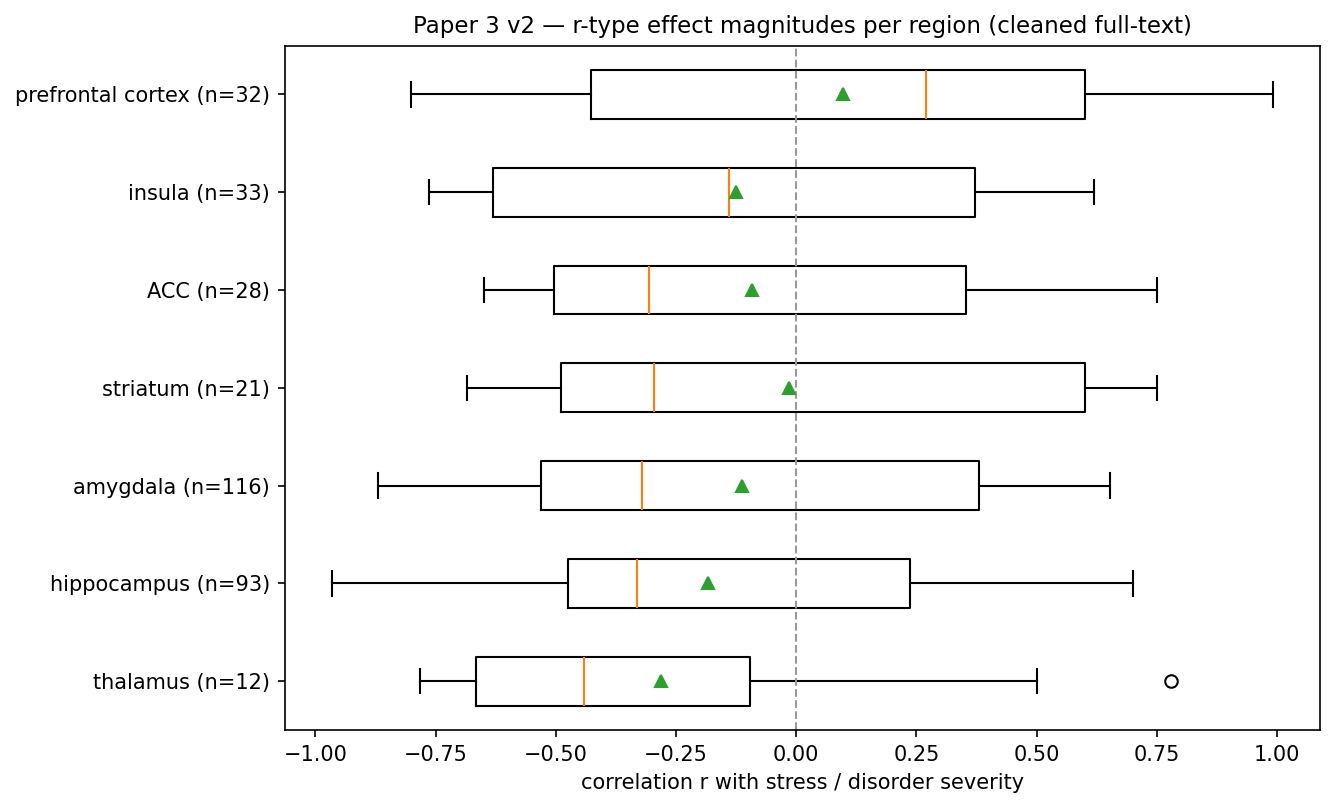
\includegraphics[width=0.85\linewidth]{figures_v2/v2_fig2_r_magnitude.png}
\caption{Distribution of $r$-type effect magnitudes per region (cleaned
full-text). Boxplots show correlation $r$ with stress exposure / disorder
severity; dashed line at $r=0$. Amygdala, hippocampus and ACC center near
$r\approx-0.3$ (moderate negative associations).}
\label{fig:rmag}
\end{figure}

\subsection{Correlation magnitudes are moderate}
Among $r$-type entries, correlations with stress exposure or disorder severity
clustered around $r\approx-0.30$ for the amygdala (median $-0.32$, $n=113$),
hippocampus ($-0.31$, $n=90$) and ACC ($-0.29$, $n=28$), indicating moderate
negative associations (Figure~\ref{fig:rmag}). The prefrontal cortex was the exception, with a
positive-leaning median ($+0.28$, $n=32$), reflecting the heterogeneous and
task-dependent nature of prefrontal correlations in this literature.

\subsection{Extraction accuracy}
On the 300-sentence validation sample, 155 sentences carried an unambiguous
lexical direction cue and entered the comparison. Against this independent label,
the model's mapped direction was correct in 146/155 cases (\textbf{94\%
accuracy}). The errors were \emph{symmetric}: 4 false ``increase'' and 5 false
``decrease'' (confusion matrix: decrease$\to$decrease 80, decrease$\to$increase
4, increase$\to$increase 66, increase$\to$decrease 5). Because directional
misclassification is balanced rather than skewed toward one pole, it is unlikely
to bias the sign tests systematically; a one-sided extraction artifact---the most
dangerous failure mode for a directional synthesis---is not present.

\subsection{Extracted magnitudes vs.\ individual-patient-data mega-analyses}
To external-validate our magnitude estimates, we compared them with the largest
individual-patient-data (IPD) mega-analyses of limbic structure, which are by
design free of publication bias. Converting our median correlations to Cohen's
$d$ ($d = 2r/\sqrt{1-r^2}$): hippocampus $r=-0.31 \to d\approx-0.65$; amygdala
$r=-0.32 \to d\approx-0.68$; ACC $r=-0.29 \to d\approx-0.61$. The corresponding
IPD estimates are markedly smaller: ENIGMA-PTSD reported hippocampus $d=-0.17$
and amygdala $d=-0.11$ (the latter not surviving multiple-comparison correction)
\cite{logue2018}, and ENIGMA-MDD reported hippocampus $d=-0.14$ (recurrent
$-0.17$) \cite{schmaal2016}. Our extracted, published-literature magnitudes thus
exceed the unbiased benchmarks by $\approx$3--4$\times$ (hippocampus) to
$\approx$6$\times$ (amygdala). The contrast is sharper for severity correlations
specifically: ENIGMA-MDD found \emph{no} association between symptom severity and
regional volume \cite{schmaal2016}, whereas our extracted severity correlations
cluster near $r\approx-0.3$. The \emph{direction} of our synthesis therefore
matches the gold standard, but its \emph{magnitude} reflects the selective
reporting of large, significant effects in the publishable literature.

\section{Discussion}

The central result is two-sided. On \emph{direction}, full-text mining is
reassuring: stress-related structural decrease in the hippocampus is recovered
with study-level directional significance ($p=6\times10^{-8}$), matching both our
abstract-level counts and consortium mega-analyses. On \emph{magnitude}, it is
revisionist: the extracted correlations ($r\approx-0.3 \approx d\approx-0.65$)
overstate the unbiased mega-analytic effects ($d\approx-0.14$ to $-0.17$) by
3--6$\times$. The agreement between abstract-level and full-text \emph{counts}
therefore does not establish that the literature is unbiased---both inherit the
same upstream publication bias, which our magnitude comparison makes visible. The
contribution of this work is thus not merely to confirm a narrative, but to show
that LLM-scale mining can \emph{quantify the gap} between the published and the
unbiased estimate.

This matters methodologically, but the lesson is the opposite of a clean
validation. One might worry that abstract-level directional counting is an
artifact of how authors phrase abstracts. Full-text counts landing in the same
direction rules out a \emph{phrasing} artifact---but it cannot rule out
\emph{publication} bias, which acts on what is published at all rather than on
wording, and which abstracts and Results sections share equally. Our comparison
with IPD mega-analyses (\S3.6) makes this concrete: both abstract-level and
full-text estimates carry the same several-fold magnitude inflation relative to
the unbiased benchmark. The practical implication is that LLM-scale mining of
published text is a reliable instrument for \emph{direction} and for
\emph{quantifying the publication-bias gap}, but not a substitute for IPD pooling
when an unbiased magnitude is the goal. A second, sobering observation is that
the amygdala structural decrease---significant at the entry level but not at the
study level---would have been over-claimed by a sentence-level analysis;
study-level aggregation is therefore not a formality but a guard against
pseudoreplicated false positives.

\subsection{Limitations}
We are deliberately conservative in framing. First, \textbf{this is not a pooled
meta-analysis}: per-study sample sizes were extractable in only $\sim$6\% of
records, precluding inverse-variance weighting; we report directional sign tests
and magnitude distributions instead. Second, \textbf{mapping yield is moderate}
($\sim$43\% of stress-context candidate sentences produced a confident mapping);
unmapped sentences are dominated by null results and non-qualifying numbers, but
some true effects are missed, so counts are lower bounds. Third,
\textbf{pseudoreplication.} Extraction is at the sentence level, so a single
study can contribute multiple entries, violating the independence assumption of a
naïve sign test. We address this by making the study the primary unit
(majority-vote direction per study $\times$ region $\times$ metric; \S2.5); the
entry-level counts are retained only for transparency, and the amygdala result
illustrates that the distinction is material, not cosmetic. Residual
non-independence remains (studies share methods, populations, and field-level
priors), so even study-level significance is not equivalent to inverse-variance
pooling. Fourth, \textbf{vote-counting is a known-limited synthesis method}: it
ignores effect magnitude and per-study precision, and with underpowered
constituent studies it can converge on the wrong conclusion as study count grows
\cite{hedges1985,borenstein2009}. Our sign tests should be read as tests of
directional consistency in the published record, not as estimates of a pooled
effect. Fifth, \textbf{the magnitudes are conditioned on publication and
significance} (the ``winner's curse''); \S3.6 quantifies this as a 3--6$\times$
gap against IPD mega-analyses, and without per-study sample sizes we cannot
construct funnel plots or apply trim-and-fill, so the median $r$ values are
upper-leaning summaries of a selected sample, not bias-corrected population
effects. Sixth, \textbf{construct conflation}: the predictor ``stress exposure /
disorder severity'' pools heterogeneous constructs (chronic stress, PTSD, MDD,
early-life adversity, cortisol, perceived stress) whose relationships with
structure plausibly differ (e.g.\ ENIGMA-MDD found no severity--volume
association); the wide IQRs in Figure~\ref{fig:rmag} are consistent with this,
and stratified synthesis by exposure type is clear future work. Seventh, the
corpus is the PMC Open Access subset, which over-represents certain journals.
These boundaries are exactly what separates this effect-size \emph{synthesis}
from a registered meta-analysis, which would require manual per-study
effect/sample-size curation on the prioritized regions.

\subsection{Conclusion}
Full-text effect-size synthesis across 384 studies recovers the \emph{direction}
of stress-related hippocampal structural decrease in the studies' own numbers,
but benchmarking against bias-free IPD mega-analyses shows the extracted
\emph{magnitudes} are inflated 3--6$\times$. LLM-scale mining of published text is
thus a reliable instrument for direction and for \emph{quantifying} the field's
publication bias---not for escaping it. We report the pipeline's validated
direction accuracy (94\%, symmetric errors), its mapping yield ($\sim$43\%), and
the absence of usable sample sizes, so that the boundary between this synthesis
and a definitive meta-analysis is explicit.

\section*{Data and Code Availability}
\begin{itemize}
\item Complete list of all included studies (PMID, title, journal, year, PMC
ID): Supplementary Table~S1.
\item Source abstracts/full texts: retrievable from PubMed/PMC via the
identifiers in Supplementary Table~S1, under each article's respective license.
\item Extraction and synthesis code (\texttt{fulltext\_hybrid\_extract.py}, the
LLM-mapping runner, and the synthesis/sign-test scripts), the exact LLM prompt
(Appendix~A), and the de-identified LLM-mapped effect-size records are publicly
available at \url{https://github.com/shoo99/ai-drug-target} (directory
\texttt{paper3/}).
\end{itemize}

\section*{Companion preprint}
This study extends the abstract-level scoping review:
Kang B. (2026), \emph{Large-Scale Scoping Review of Chronic Stress-Induced Brain
Changes via LLM-Powered Extraction of 9,585 Studies}, Research Square,
\href{https://doi.org/10.21203/rs.3.rs-9884522/v1}{10.21203/rs.3.rs-9884522/v1}.

\section*{Acknowledgments}
LLM extraction was performed on a distributed CPU cluster (no GPU). Manuscript
preparation was assisted by Claude (Anthropic). The author takes full
responsibility for all scientific content.

\section*{Conflict of Interest}
The author declares no conflicts of interest.

\appendix
\section*{Appendix A. LLM extraction prompt (verbatim)}
Each candidate sentence was wrapped in the chat template
\texttt{<|im\_start|>user ... <|im\_end|><|im\_start|>assistant} with a
pre-closed \texttt{<think></think>} block (no-think mode) and the following
one-shot example and instruction:

\small
\begin{verbatim}
Example 1 (map: stress->region effect) —
Sentence: "Patients with PTSD showed reduced hippocampal volume vs controls
(Cohen's d=-0.45), and amygdala activation correlated with cortisol (r=0.38)."
Output: [{"brain_region":"hippocampus","metric":"volume","direction":"decrease",
"value":-0.45,"measure_type":"d"},{"brain_region":"amygdala",
"metric":"activation","direction":"positive_correlation","value":0.38,
"measure_type":"r"}]

[the candidate sentence + its regex-detected numbers are inserted here]

This sentence is FROM A CHRONIC-STRESS / STRESS-DISORDER STUDY (PTSD,
depression/MDD, early-life stress, trauma, high cortisol), so a brain-region
group difference or change reported here IS the stress/disorder effect — MAP IT.
Map a number when it quantifies a BRAIN REGION'S metric (volume, GMV, thickness,
activation, connectivity, FA, metabolite) as: patients vs controls, stressed vs
non-stressed, a within-patient change, or a correlation with a stress/severity
measure. direction = how the region's metric goes in the PATIENT/STRESSED/
higher-severity state (decrease/increase/positive_correlation/
negative_correlation/null). DO NOT map regression predictors (age, sex,
education, medication), task-performance correlations, scanner/coordinate
numbers, or protective-factor effects. Output ONLY a JSON array of
{brain_region, metric, direction, value, measure_type}; [] if none qualify.
\end{verbatim}
\normalsize

\begin{thebibliography}{9}
\bibitem{kang2026scoping} Kang B. Large-Scale Scoping Review of Chronic
Stress-Induced Brain Changes via LLM-Powered Extraction of 9,585 Studies. {\it
Research Square} (2026). DOI: 10.21203/rs.3.rs-9884522/v1.
\bibitem{logue2018} Logue MW, van Rooij SJH, Dennis EL, et al. Smaller
Hippocampal Volume in Posttraumatic Stress Disorder: A Multisite ENIGMA-PGC
Study. {\it Biol Psychiatry} 2018;83(3):244--253.
doi:10.1016/j.biopsych.2017.09.006.
\bibitem{schmaal2016} Schmaal L, Veltman DJ, van Erp TGM, et al. Subcortical
brain alterations in major depressive disorder: findings from the ENIGMA Major
Depressive Disorder working group. {\it Mol Psychiatry} 2016;21:806--812.
doi:10.1038/mp.2015.69.
\bibitem{hedges1985} Hedges LV, Olkin I. {\it Statistical Methods for
Meta-Analysis}. Academic Press, 1985.
\bibitem{borenstein2009} Borenstein M, Hedges LV, Higgins JPT, Rothstein HR.
{\it Introduction to Meta-Analysis}. Wiley, 2009.
\end{thebibliography}

\end{document}
